% ============================================================
%  Research Findings  --- WITH FIGURES
%
%  This is findings.tex plus three figures from the real experiments.
%  Figures live in ./proposal_figures/ (ship that folder alongside this file).
%
%  REQUIRES in the preamble (proposal_single.tex already loads graphicx):
%     \usepackage{graphicx}
%     \graphicspath{{proposal_figures/}}   % <- add this line
%
%  SHARING WITH WEB CLAUDE (read this):
%   - A .tex only *references* images by path; sending the .tex alone does
%     NOT carry the pictures. Web Claude also cannot compile LaTeX, so it
%     will not render \includegraphics.
%   - To let web Claude actually SEE the figures, upload the three PNGs in
%     ./proposal_figures/ as image attachments too (web Claude has vision),
%     OR compile this to a PDF first (e.g. on Overleaf) and upload the PDF.
%   - The captions below are written to be self-contained, so even text-only
%     they convey what each figure shows.
% ============================================================

\section{Research Findings}
\label{sec:findings}

This chapter reports what we have learned so far, in two parts. We first
consolidate the conceptual findings that the recent literature makes available
to us---chiefly, that the task-understanding bottleneck is real, measurable, and
addressable by an \emph{explicit} task representation rather than a
language-mediated or implicitly-reasoned one (Section~\ref{sec:findings:lit}).
We then report a preliminary empirical study in which we actually learn such a
representation and probe whether it is attainable, verifiable, and
discriminative (Section~\ref{sec:findings:study}). The study supersedes the
set-membership / convex-cone framing of the earlier abstract: rather than
committing to a particular geometry of the embedding space up front, we treat
the central object as \emph{an explicit, separable, learnable task
representation} and measure it directly.

\subsection{Findings from the Literature}
\label{sec:findings:lit}

Three findings from recent work jointly motivate and constrain our direction.

\paragraph{F1 --- The task-understanding bottleneck is real and quantifiable.}
LIBERO-Plus~\cite{liberoplus} demonstrates that state-of-the-art VLAs are
disproportionately sensitive to visual features while remaining largely
insensitive to the language instruction, producing task confusion, looping, and
disregard for explicit intent. The important methodological consequence---which
we adopt---is that ``does the model know which task it is doing?'' is not a soft
qualitative property but something that can be \emph{operationalized and
measured}. This reframes task understanding from an assumption into a testable
quantity, and it is the premise on which our Experiment~1 rests.

\paragraph{F2 --- Existing remedies route task identity through lossy channels.}
Hierarchical planners ($\pi_{0.5}$~\cite{pi05}, Hi Robot~\cite{hirobot}) preserve
natural language as the inter-layer medium, so the ambiguity of an instruction
such as ``pick up the cup'' is carried, not resolved, by the channel itself.
Chain-of-thought VLAs (CoT-VLA~\cite{cotvla}) instead distribute task identity
across an autoregressive reasoning trace, where it is neither localized nor
inspectable. Across both families, task identity is never instantiated as a
separable, verifiable representation. This is the gap our work targets.

\paragraph{F3 --- Explicit, temporally-grounded task representations are
learnable.} Crucially, the literature also shows the positive direction is
feasible. Contrastive and successor-feature representation learning can recover
task structure as an explicit embedding: Temporal Representation
Alignment~\cite{tra} shows that aligning representations along temporal/successor
structure yields \emph{emergent compositionality} in instruction following, and
RS-CL~\cite{rscl} learns task-discriminative embeddings via a contrastive
objective. These results tell us that an explicit task representation supplied to
the policy is not only desirable (F1, F2) but attainable in principle---and they
point to representation-alignment objectives, rather than a hand-specified
embedding geometry, as the right tool. Our preliminary study is an instance of
exactly this: an intention-conditioned occupancy embedding learned over robot
trajectories.

\subsection{Preliminary Study: An Explicit Task Embedding Is Attainable and Verifiable}
\label{sec:findings:study}

\paragraph{Setup.} We learn an explicit per-timestep task representation
$z = q(z \mid s, a)$ as the intention variable of an intention-conditioned
occupancy model~\cite{infom}: $z$ summarizes the discounted \emph{future}
trajectory from a state, so it is a temporally-grounded encoding of ``what task
is being executed,'' in the same spirit as the successor-feature representations
of F3. Observations are multimodal: a frozen ImageNet ResNet-34 image feature
($512$-d) concatenated with proprioceptive state, and---in one variant---a
sentence-embedding of the task instruction ($384$-d). We study two benchmarks:
all $65$ Robocasa atomic manipulation tasks, and the $10$ instruction tasks of
LIBERO-goal. To judge representation quality without conflating it with policy
success, we use two complementary diagnostics: (i) \emph{task separability}
(Fisher trace-ratio and $k$-NN task-classification accuracy over the embedding),
and (ii) a \emph{trajectory-fidelity} diagnostic that correlates embedding
distance with the geometric DTW distance between the underlying raw
state/action trajectories (Spearman~$\rho$).

\paragraph{R1 --- An explicit task embedding is attainable and discriminative.}
The learned embedding separates tasks far above chance. On the $65$-way Robocasa
pool, $k$-NN task accuracy reaches $\sim\!43\%$ (chance~$\approx\!1.5\%$;
$\sim\!29\times$), with a Fisher trace-ratio of $\sim\!0.19$--$0.21$. On the
cleaner $10$-task LIBERO-goal benchmark the structure is sharper still: the
language-conditioned model forms visually distinct $t$-SNE clusters per
instruction (Fisher~$0.358$, vs.\ $0.343$ for the state-only model;
Figure~\ref{fig:tsne}). An explicit, separable task representation is therefore
\emph{attainable}---the core feasibility claim behind contribution~(iii) of the
proposal.

\begin{figure}[t]
  \centering
  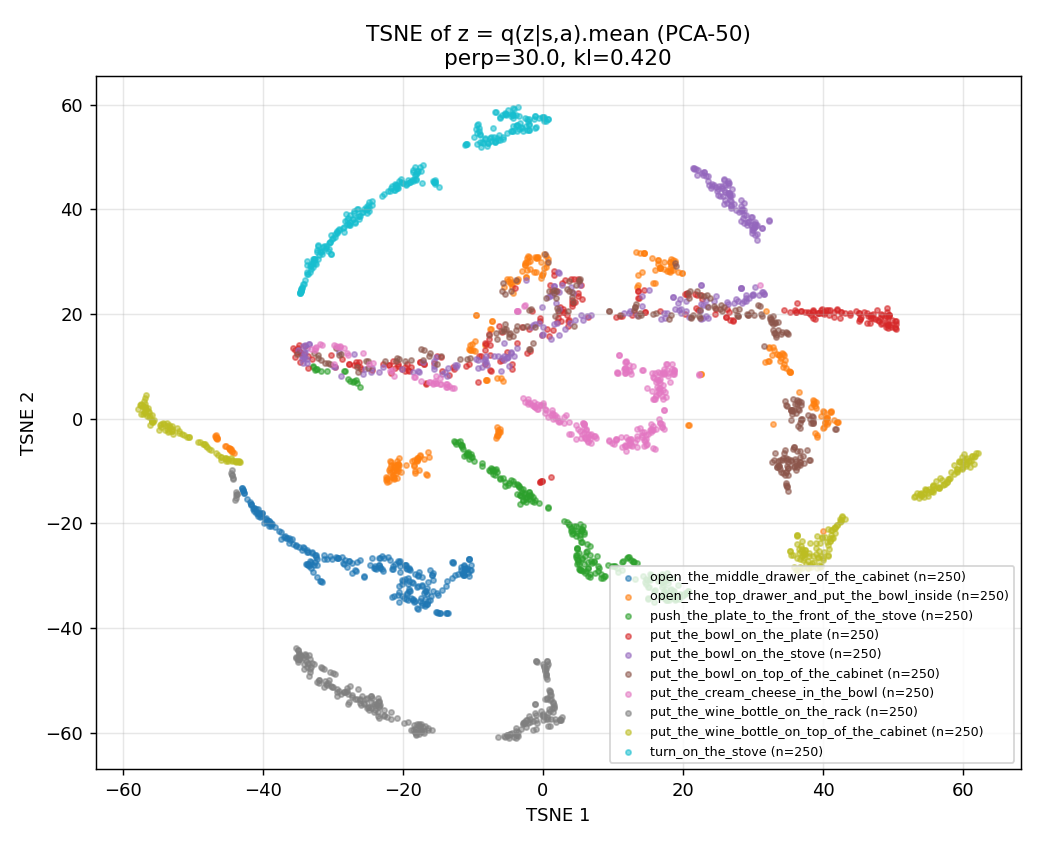
\includegraphics[width=0.74\linewidth]{fig_libero_tsne.png}
  \caption{\textbf{The learned task embedding separates tasks (R1).} $t$-SNE of
  the intention embedding $z=q(z\mid s,a)$ from the \emph{language-conditioned}
  LIBERO-goal model (latest checkpoint, $500$k steps), colored by the $10$
  ground-truth instructions. Without any task label in the objective, the
  embedding forms distinct per-instruction clusters (Fisher trace-ratio
  $0.358$); the residual overlap is concentrated in the semantically confusable
  bowl-placement family (same pick motion, different destination), which is
  exactly where language conditioning helps most (R3).}
  \label{fig:tsne}
\end{figure}

\paragraph{R2 --- The representation is verifiable independently of end-task
success.} Our trajectory-fidelity diagnostic cleanly separates good
representations from bad ones, which is what makes Experiment~3 well-posed.
Models whose embedding is trained on a tractable target attain within-task
embedding$\leftrightarrow$trajectory $\rho \approx 0.5$--$0.6$, whereas an
ablation that forces $z$ to additionally reconstruct the erratic image features
collapses to $\rho \approx 0.18$ (with \emph{negative} correlation on the action
channel). A task-agnostic, all-pairs view of the diagnostic is shown in
Figure~\ref{fig:traj}: on LIBERO-goal, embedding distance and geometric
trajectory distance are positively correlated across \emph{every}
distance-reduction $\times$ embedding-metric combination (Spearman
$\rho\!\approx\!0.45$--$0.62$ at convergence). The trend with training is
benchmark-dependent---on Robocasa the correlation is strongest \emph{early}
(peaking around $50$--$150$k steps, tracking the Fisher separability), whereas on
the cleaner LIBERO-goal it strengthens through training and is sustained around
$\rho\!\approx\!0.6$. The same lens shows the embedding encodes not just task
identity but intra-task execution variation (strong \emph{within} a task, weak
\emph{across} tasks). The headline consequence for the proposal is
methodological: \textbf{we already have a working, label-free way to verify that
a task representation is meaningful}, so Experiment~3 is de-risked.

\begin{figure}[t]
  \centering
  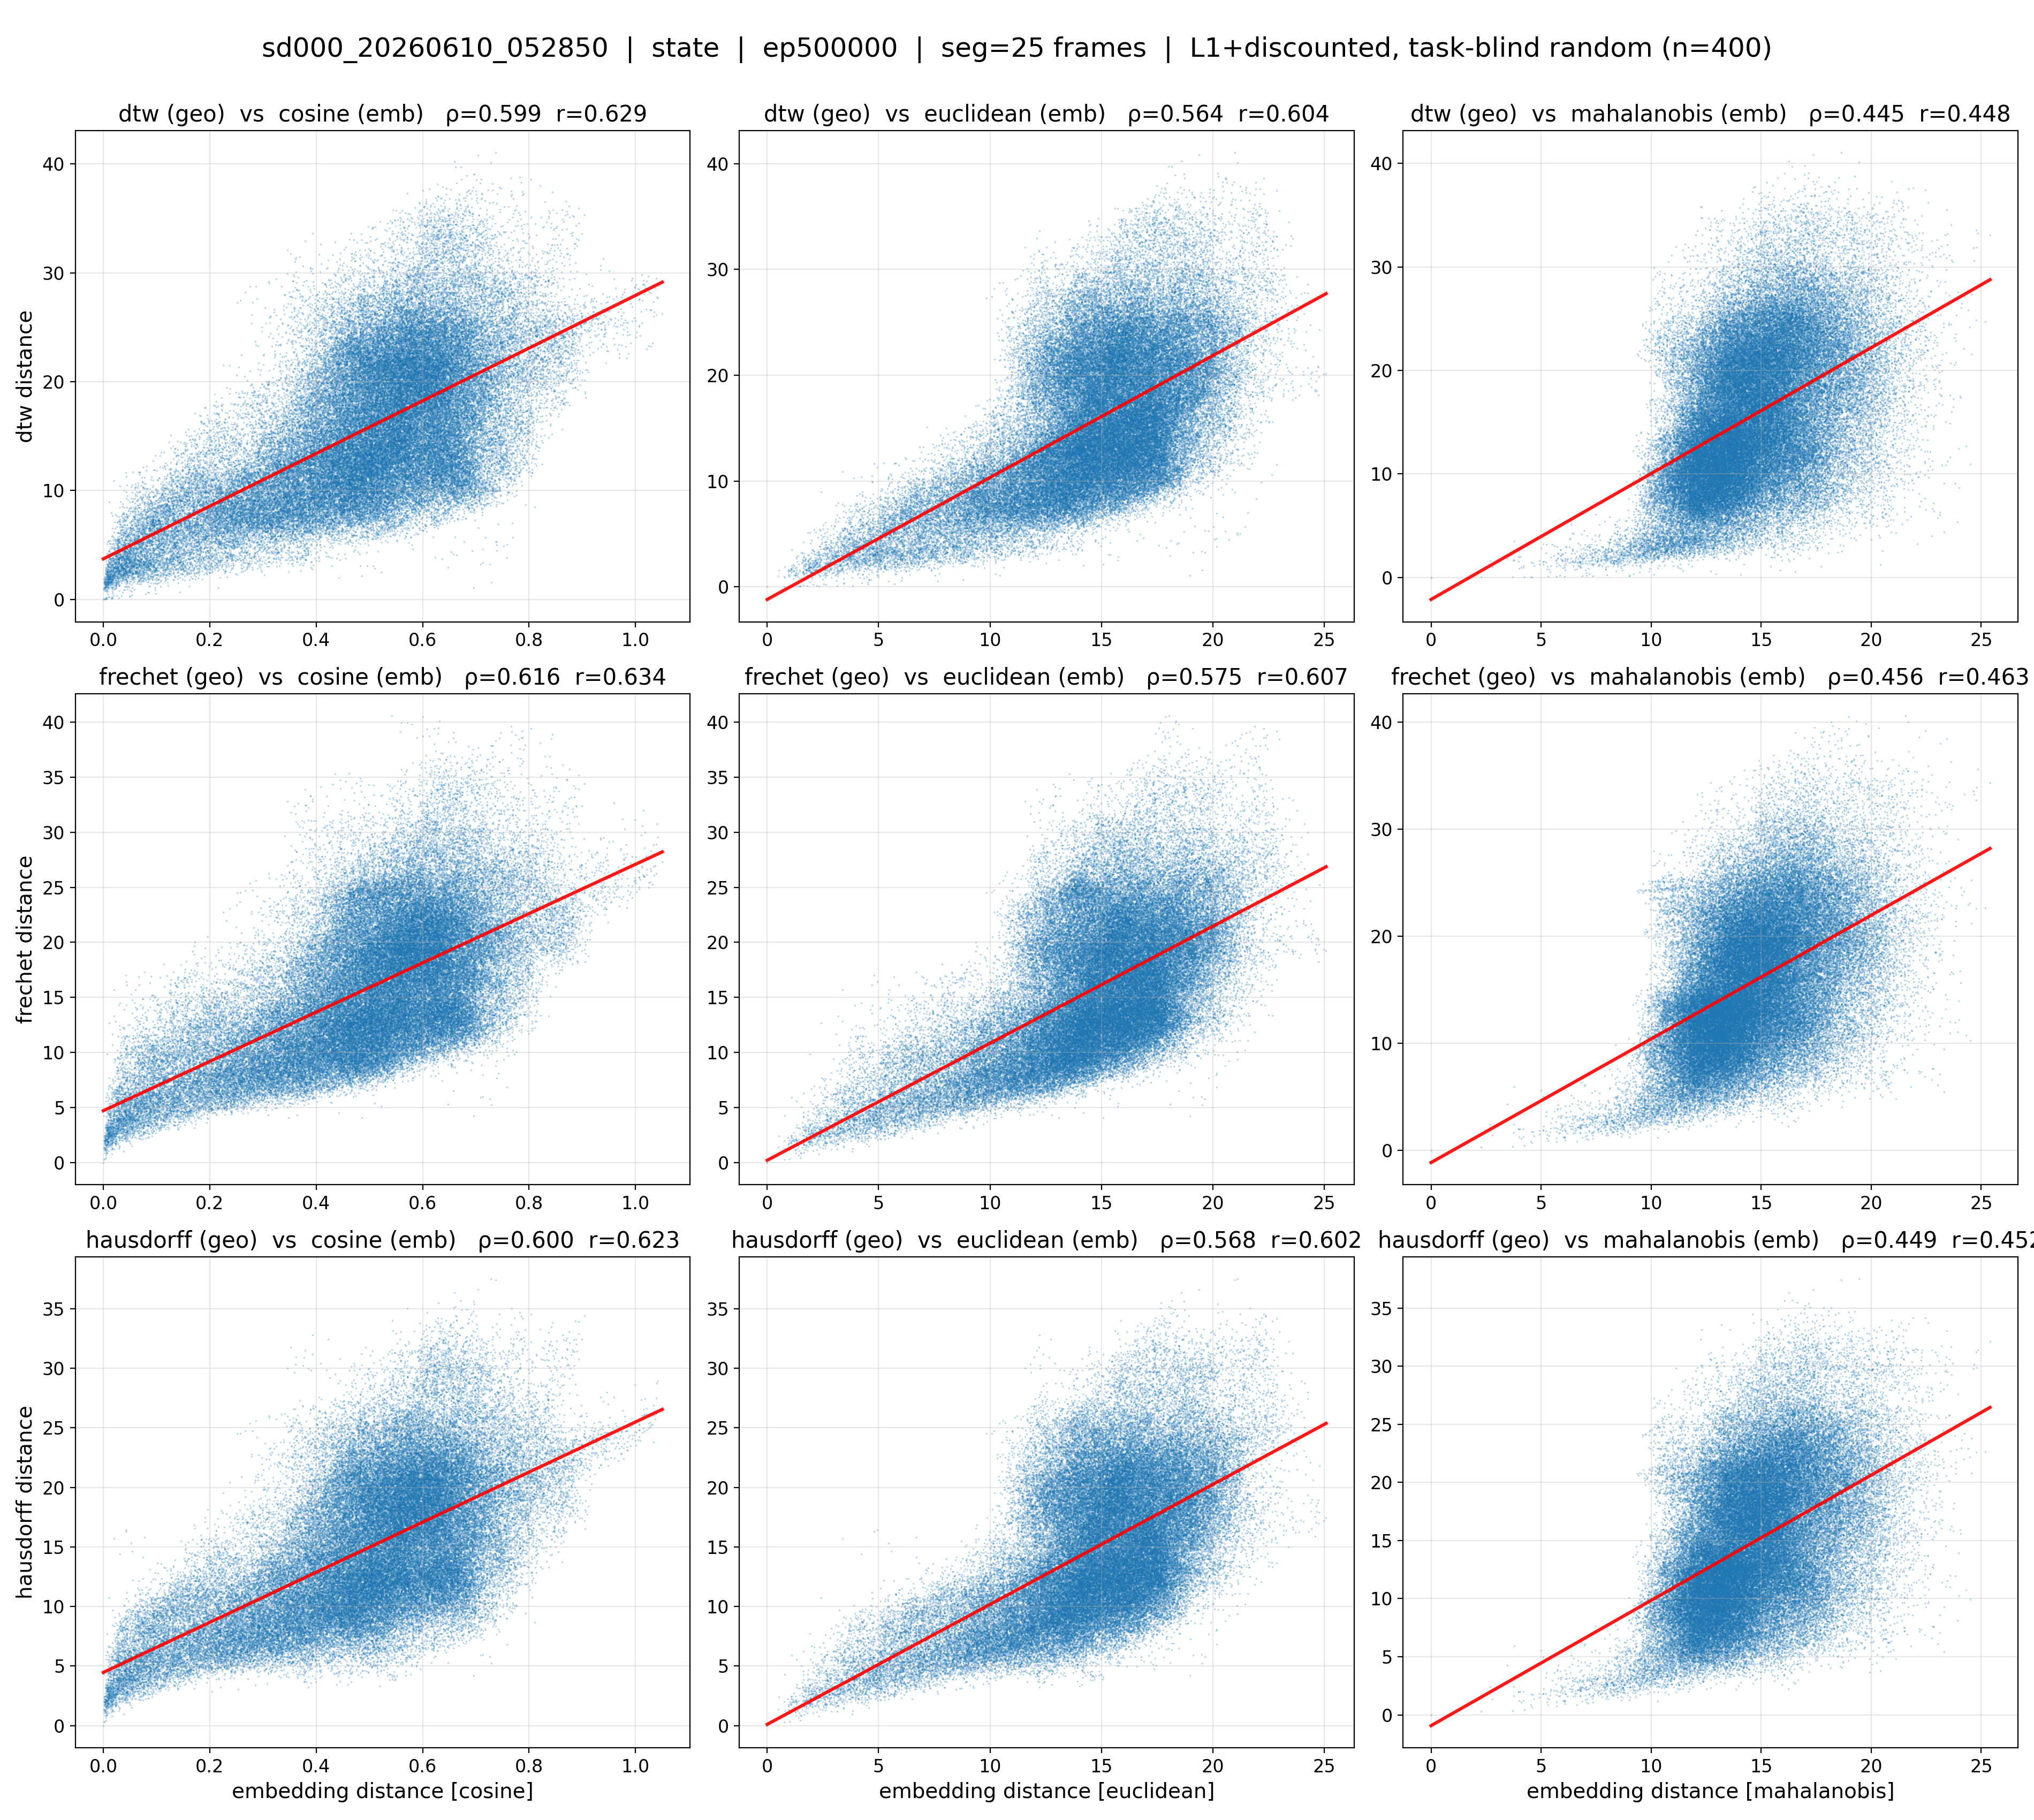
\includegraphics[width=\linewidth]{fig_dtw_fit.png}
  \caption{\textbf{A label-free verification of representation quality (R2).}
  Task-agnostic, all-pairs relationship between embedding distance ($x$) and
  geometric trajectory distance ($y$) for the language-conditioned LIBERO-goal
  model at convergence ($500$k steps, segment length $25$, $L_1$/discounted).
  Rows are the three geometric reductions (DTW / Fr\'echet / Hausdorff); columns
  are the three embedding metrics (cosine / Euclidean / Mahalanobis). Each panel
  shows the OLS fit (red) with Spearman $\rho$ and Pearson $r$ annotated. The
  correlation is positive and stable across all nine combinations
  ($\rho\!\approx\!0.45$--$0.62$, strongest for cosine/Euclidean embedding
  distance), confirming the embedding tracks trajectory geometry. For contrast, a
  degenerate ablation that forces $z$
  to also reconstruct image features collapses this correlation to
  $\rho\!\approx\!0.18$---so the diagnostic discriminates good representations
  from bad ones without any task label.}
  \label{fig:traj}
\end{figure}

\paragraph{R3 --- Explicit conditioning resolves exactly the ambiguous cases.}
Adding the language instruction to the representation sharpens \emph{task
identity} precisely where intent is ambiguous. On LIBERO-goal, per-demonstration
$k$-NN agreement rises on all ten tasks (mean $0.857 \to 0.898$), with the
largest gains concentrated on the confusable bowl-placement family
(``put the bowl on the \{plate, cabinet, stove\}''---identical pick motion,
different destination), whose confidence climbs from $\sim\!0.65$--$0.74$ toward
the $\sim\!0.93$--$1.0$ of already-distinct tasks. Notably, language improves
\emph{which task} the embedding thinks it is doing without much changing the
geometric trajectory correlation---direct evidence that explicit task
conditioning attacks the ambiguity bottleneck (F1, F2) rather than merely
fitting trajectories better.

\paragraph{R4 --- Embedding fidelity is structured, and points at where to
improve.} Representation quality is not uniform across tasks
(Figure~\ref{fig:rank}). Constrained, low-variance motions embed
tightly---articulated tasks (open/close/slide, $\rho \approx 0.53$) and knob
tasks (turn on/off, $\rho \approx 0.52$)---while free-space, high-variance
behaviors embed poorly---pick-and-place ($\rho \approx 0.39$) and especially
navigation ($\rho \approx 0.25$), with counter-to-microwave pick-place the worst
($\rho \approx -0.05$). The interpretation is mechanistic: when motion is tightly
constrained, a single future-summarizing vector predicts the trajectory well;
when the task admits many divergent free-space paths, no single $z$ can. This
both validates the diagnostic (it recovers an intuitive difficulty ordering) and
tells us where representation improvement must be aimed---the compositional,
free-space manipulation regime that long-horizon tasks are made of.

\begin{figure}[t]
  \centering
  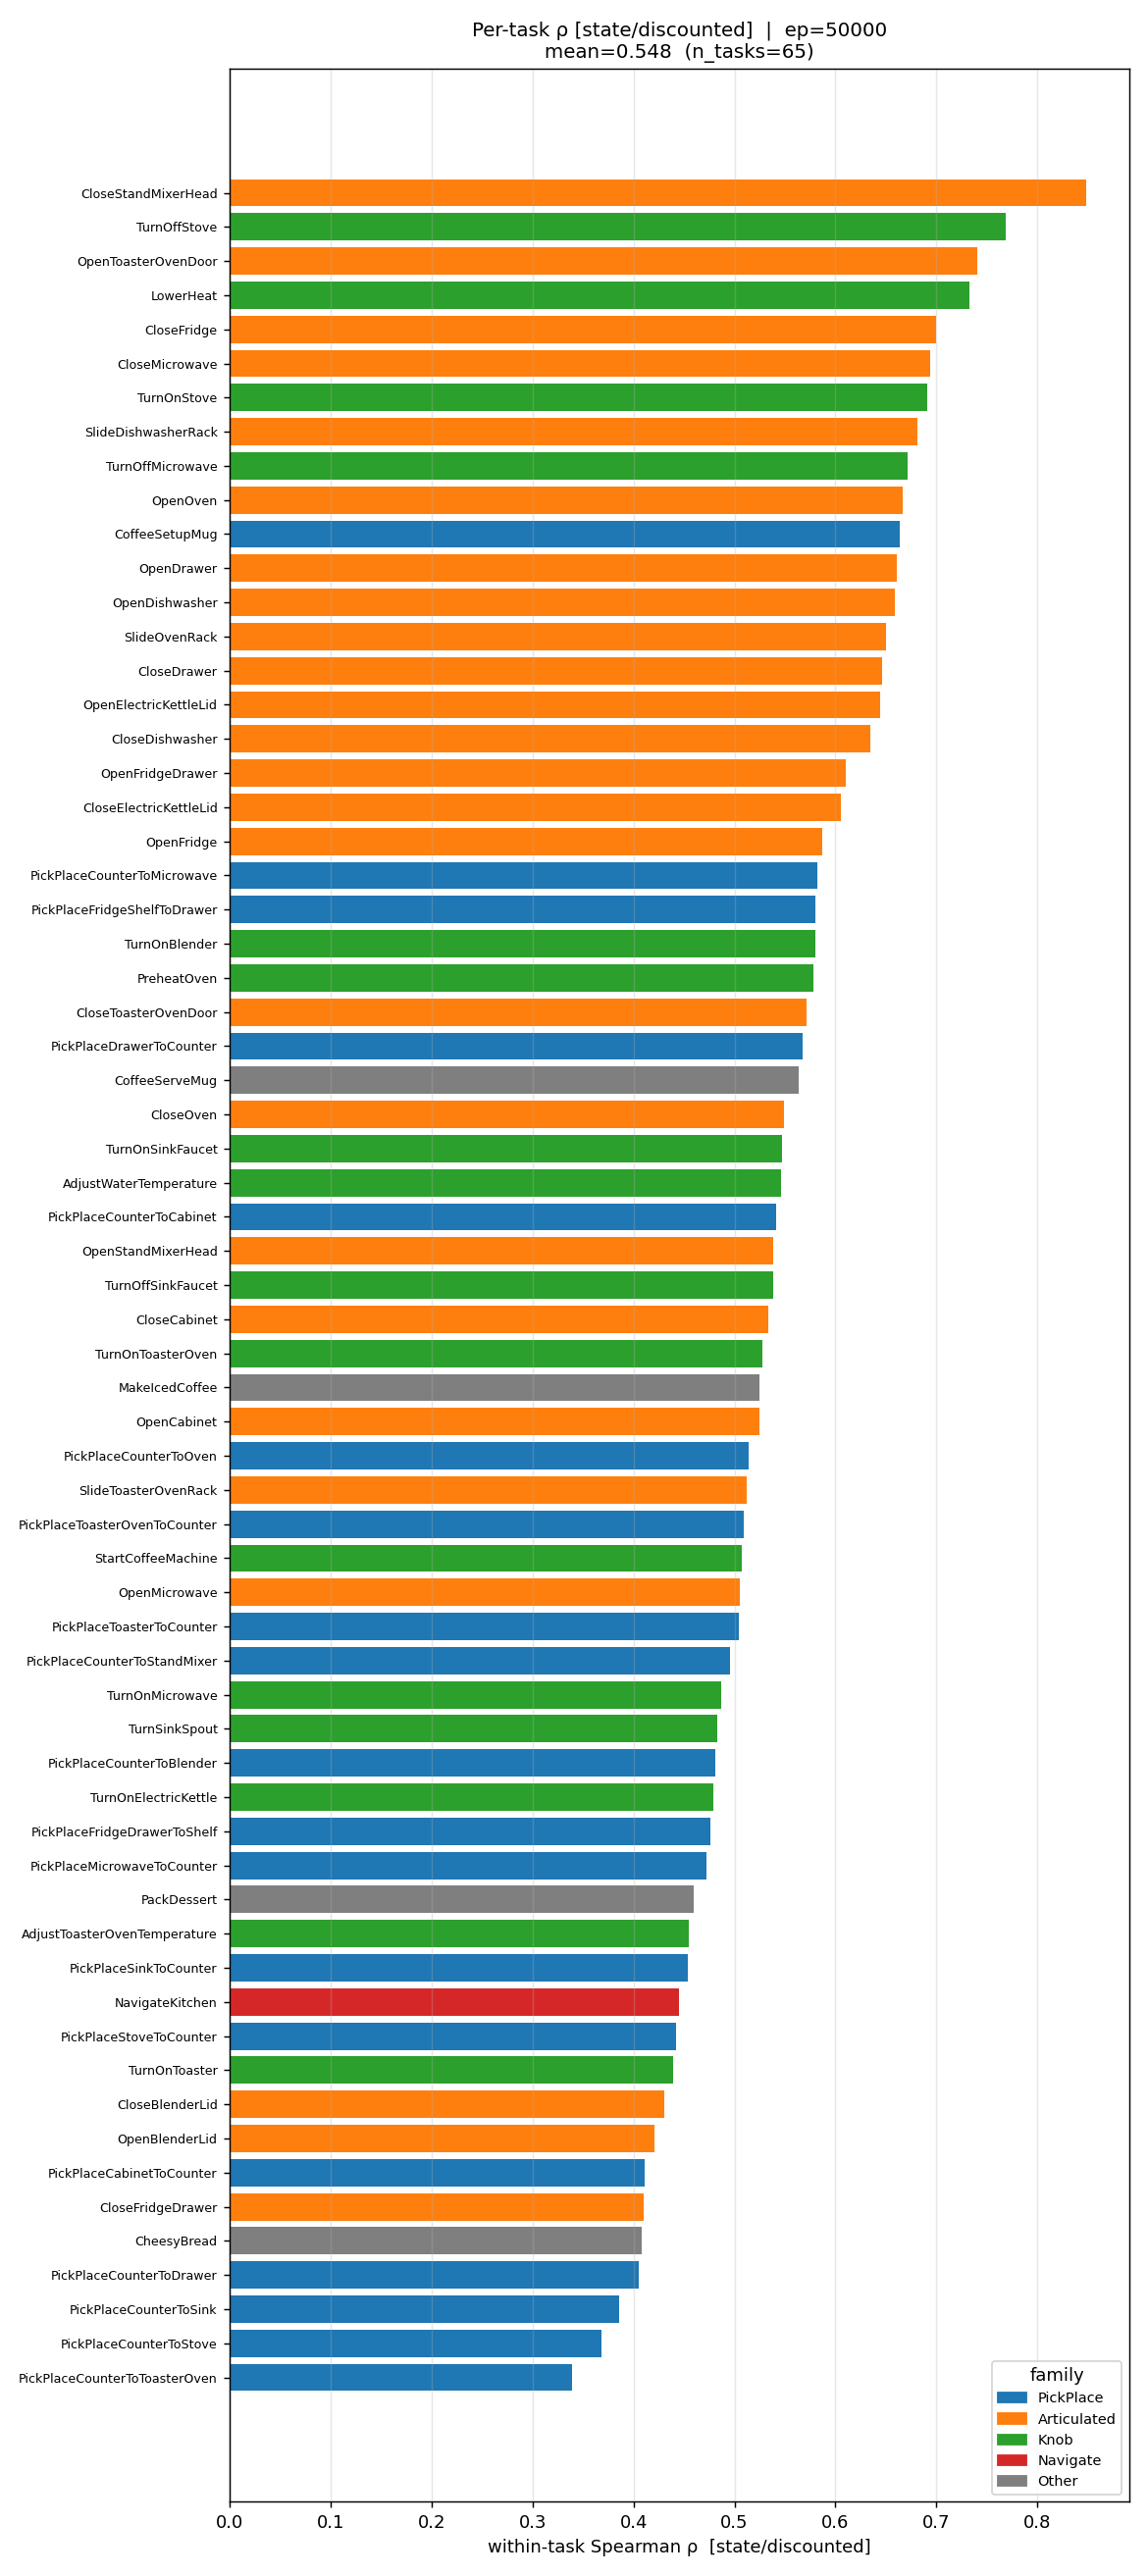
\includegraphics[width=0.62\linewidth]{fig_task_rank.png}
  \caption{\textbf{Embedding fidelity is structured by task type (R4).} Per-task
  within-task embedding$\leftrightarrow$trajectory Spearman $\rho$ for all $65$
  Robocasa tasks, colored by motion family (mean $0.548$). Constrained
  articulated and knob tasks (top) embed tightly; free-space pick-place and
  navigation tasks (bottom) embed poorly. The ordering identifies exactly which
  regime---compositional, free-space manipulation---the proposed module must
  improve.}
  \label{fig:rank}
\end{figure}

\paragraph{R5 --- Composition leaves a trace in the embedding.} As a first probe
of compositionality, we check whether held-out \emph{composite} task
demonstrations traverse the atomic-skill clusters of the embedding. They do, in
the expected qualitative pattern, though with low $k$-NN vote confidence
($\sim\!0.21$) that is unsurprising for a $65$-way space and a frozen visual
backbone. We read this as encouraging-but-preliminary evidence that an explicit
task embedding can support the kind of subtask decomposition long-horizon
control needs---and, together with the flat separability we observe across
training, as motivation to move from frozen features to a learned (end-to-end)
visual encoder in the next phase.

\subsection{Implications for the Proposal}
\label{sec:findings:implications}

These findings shift the proposal's center of gravity in three concrete ways.
First, they \textbf{de-risk Experiment~3}: a label-free verification methodology
(task separability $+$ trajectory-fidelity correlation, with a canonical
task-agnostic, $L_1$/discounted distance configuration) already exists and
discriminates good representations from bad ones. Second, they \textbf{refine the
method}: the current direction is to learn an explicit, temporally-grounded task
representation via representation-alignment / contrastive objectives in the
successor-feature spirit (F3,~\cite{tra,infom}), conditioned multimodally on
vision, proprioception, and language---\emph{not} to impose a convex-cone or
other fixed set geometry, which we now treat as out of scope. Third, they
\textbf{localize the hard case}: free-space, compositional manipulation is where
the representation is weakest (R4) and therefore where the proposed module must
prove its value, which sharpens the task selection for Experiment~2. In short,
the premise the proposal set out to defend---that task identity can be made an
explicit, separable, and \emph{verifiable} representation---is supported by
direct measurement, and the open work is to convert that representation into
action-generation gains on the long-horizon, compositional tasks where it is
currently thinnest.

% ============================================================
%  NEW BIBITEMS  --- move these into thebibliography when merging.
%  TODO(author): verify arXiv ids / author lists before submission.
% ============================================================
% \bibitem{tra} V. Myers et al. \emph{Temporal Representation Alignment:
%   Emergent Compositionality in Instruction Following with Successor Features.}
%   arXiv, 2025.  % TODO: confirm authors + arXiv id
%
% \bibitem{infom} \emph{Intention-Conditioned Flow Occupancy Models (InFOM).}
%   2025.  % TODO: confirm authors + venue/arXiv id (method basis for q(z|s,a))
